\chapter{Projekt systemu (Magdalena Solecka)}
\par System postanowiono podzielić na następujące komponenty:
\begin{itemize}
\item Po stronie serwera:
\begin{itemize}
\item podsystem planowania (ang. Planning subsystem),
\item podsystem wyszukiwania (ang. Search subsystem),
\item podsystem zarządzania danymi użytkownika (ang. User Data Management Subsystem),
\item podsystem polecający (ang. Recommendation Subsystem),
\item podsystem usług społecznościowych (ang. Social Services Subsystem),
\item podsystem zarządzania (ang. Management Subsystem).
\end{itemize}
\item Po stronie aplikacji mobilnej:
\begin{itemize}
\item GUI,
\item prezenter (ang. Presenter),
\item podsystem zarządzania plikami (ang. File Management Subsystem),
\item podsystem skanowania (ang. Scanning Subsystem).
\end{itemize}
\end{itemize}
\par Kontakt klienta mobilnego z aplikacją serwerową zaplanowano poprzez interfejs komunikacji (ang. communication interface). Zależności pomiędzy podsystemami zostały przedstawione na diagramie (rys.~\ref{fig:subsystems}).

\indent\newline
\begin{figure}[h]
\centering
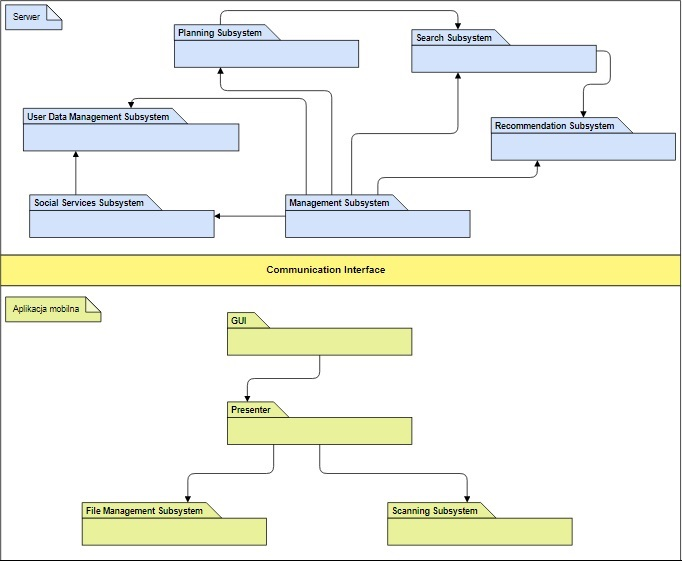
\includegraphics[width=0.9\textwidth]{subsystems}
\caption{Diagram komponentow systemu.}
\label{fig:subsystems}
\end{figure}

\FloatBarrier

\section{Scenariusze użycia}
\par Zaprojektowano scenariusze użycia w celu dokładnego określenia sposobów, na które użytkownicy będą korzystać z aplikacji. Wyróżniono najważniejsze:
\begin{enumerate}
  \item Stworzenie planu dnia.
  \item Wygenerowanie planu dnia.
  \item Stworzenie planu podróży.
  \item Interakcje z innymi użytkownikami aplikacji.
  \item Interakcje serwera z aplikacją w czasie trwania podróży.
\end{enumerate}

\FloatBarrier
\subsection{Stworzenie planu dnia (Magdalena Solecka)}
\par Martyna widzi pusty ekran planu dnia. Wpisuje miasto docelowe wyjazdu -- Paryż. Wybiera przycisk "+" i wybiera atrakcje. Ukazuje się przed nią ekran wyszukiwania ze znakiem wyszukiwania, a po chwili z wynikami wyszukiwania w formie listy atrakcji. Wybiera jeden z elementów listy – katedra Notre Dame i czyta jej opis. Wybiera przycisk "Dodaj". Widzi ponownie ekran planu Dnia z dodaną przez siebie atrakcją. Wybiera w ten sposób kilka kolejnych atrakcji. Ponownie wybiera przycisk "+" i wybiera restauracje. Ponownie widzi ekran wyszukiwania z listą restauracji. Wybiera pasujący jej obiekt i przy użyciu przycisku "Dodaj" zostaje on dodany do  planu dnia który ponownie wyświetla się przed nią. Użytkownik wybiera przycisk "Ułóż" i czeka aż aplikacja zakończy obliczanie najbardziej optymalnej trasy. Po kilku sekundach plan dnia jest już gotowy. Martyna stwierdza jednak że potrzebuje w ciągu dnia odpoczynku dlatego postanawia przesunąć zwiedzanie katedry Notre Dame na następny dzień. Wybiera element z katedrą i przycisk "Przenieś", a następnie numer dnia podróży. Następnie stwierdza, że właściwie nie interesuje jej sztuka sakralna, więc usuwa element z planu przesuwając go w prawo.

\noindent\newline Warunki początkowe:
\begin{enumerate}
  \item Użytkownik jest zalogowany.
  \item Aplikacja ma dostęp do internetu.
  \item Użytkownik wybrał opcję stwórz plan dnia.
\end{enumerate}

\noindent\newline
\begin{figure}[h]
\centering
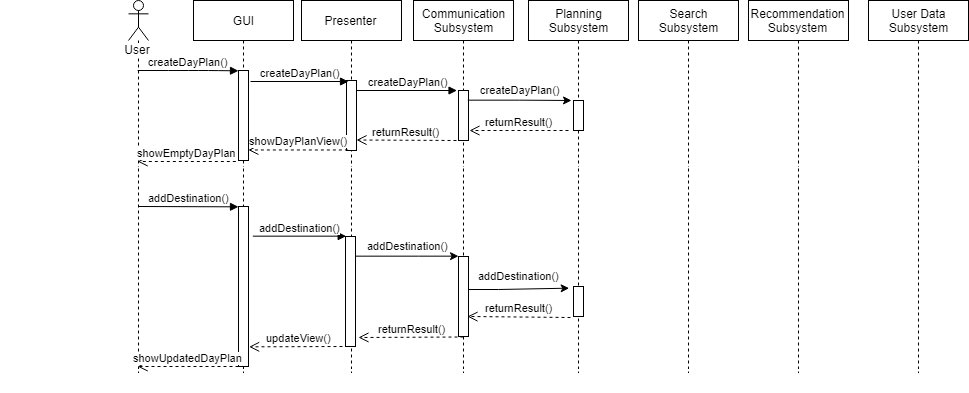
\includegraphics[width=0.85\textwidth]{dayPlan1}
\caption{Tworzenie planu dnia(1).}
\label{fig:dayPlan1}
\end{figure}
\\
\par
\noindent\newline
Warunki końcowe:
\begin{enumerate}
  \item Użytkownik stworzył plan dnia.
\end{enumerate}

\begin{figure}[h]
\centering
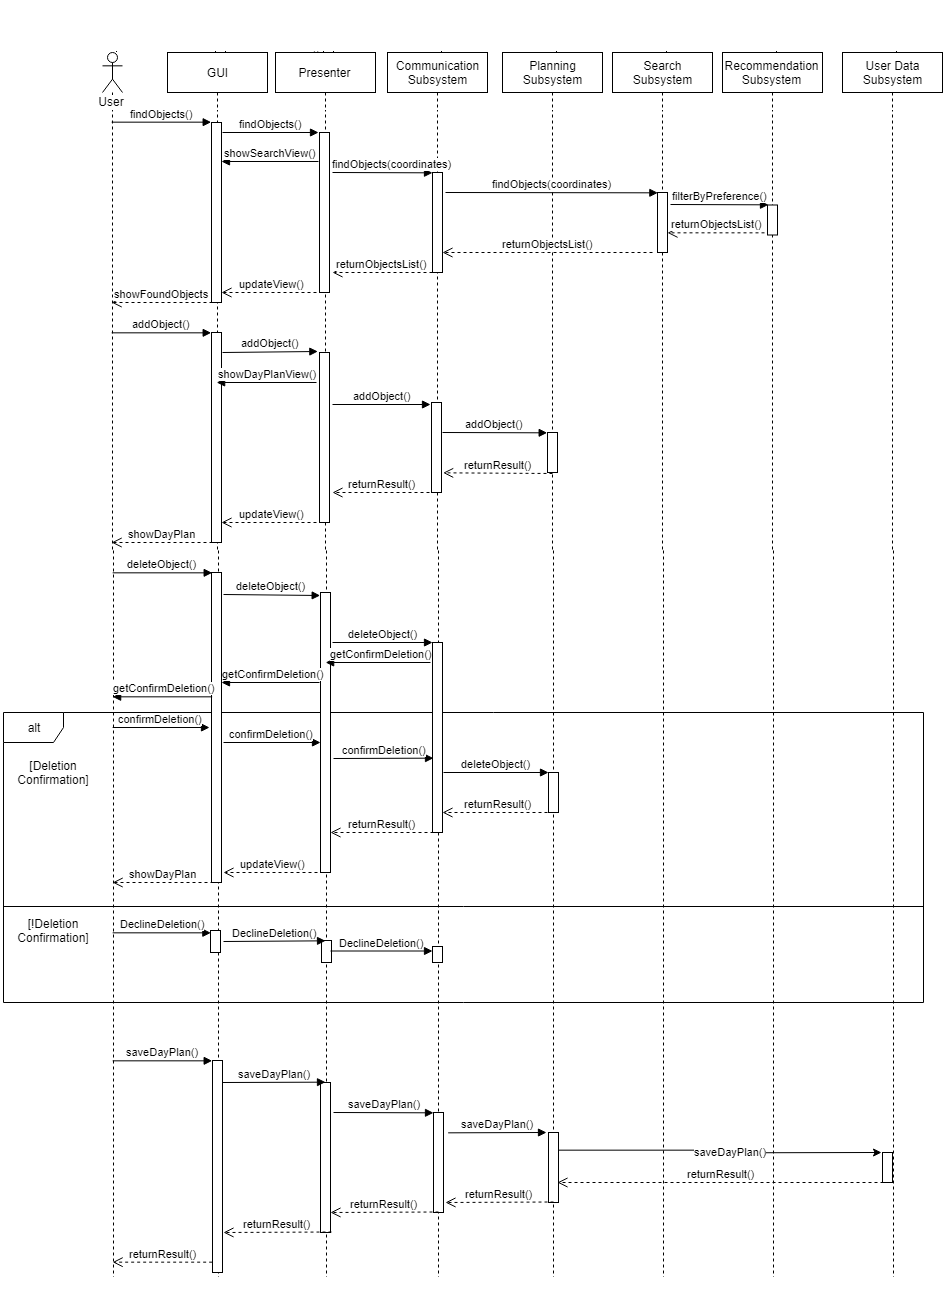
\includegraphics[width=0.9\textwidth]{dayPlan2}
\caption{Tworzenie planu dnia(2).}
\label{fig:dayPlan2}
\end{figure}

\FloatBarrier
\subsection{Wygenerowanie planu dnia (Anna Malizjusz)}
\par Martyna stworzyła wyjazd, lecz nie ma pomysłu na spędzenie dnia. Wybiera w aplikacji swoją podróż, po czym generuje przyciskiem plan dnia. Zostaje wyświetlony rezultat, który może dowolnie modyfikować. (rys.~\ref{fig:generateDayPlan}).\\\\

\noindent Warunki początkowe:
\begin{enumerate}
  \item Użytkownik jest zalogowany.
  \item Aplikacja ma dostęp do internetu.
  \item Użytkownik wybrał podróż.
\end{enumerate}
\par
\noindent\newline
Warunki końcowe:
\begin{enumerate}
  \item Wyświetlono proponowany plan podróży.
\end{enumerate}

\noindent\newline
\begin{figure}[h]
\centering
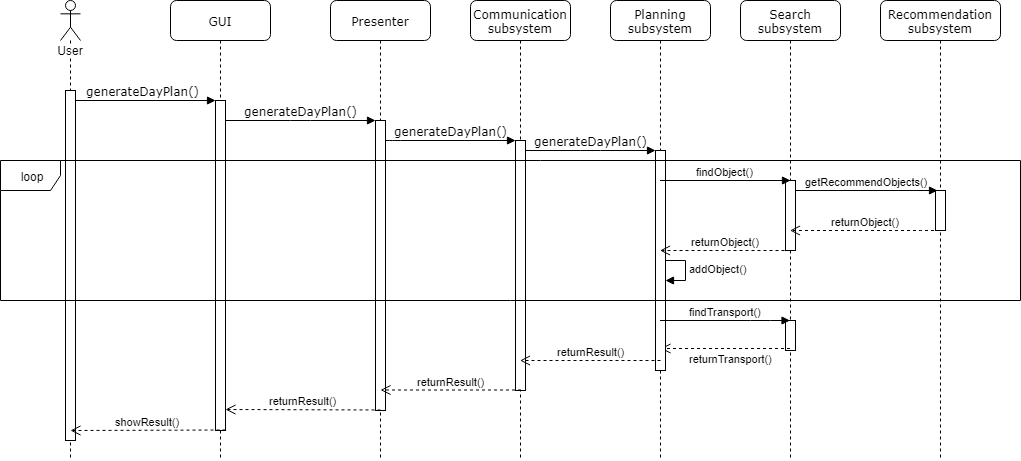
\includegraphics[width=\linewidth]{generateDayPlan}
\caption{Generowanie planu dnia.}
\label{fig:generateDayPlan}
\end{figure}

\FloatBarrier
\subsection{Interakcje z innymi użytkownikami aplikacji (Anna Malizjusz)}
\par Martyna wyjeżdża na wakacje razem z~koleżanką, więc chce udostępnić jej swój plan podróży. Zaprasza nowego użytkownika do skorzystania z aplikacji (rys.~\ref{fig:inviteFriend}), po czym dodaje znajomego (rys.~\ref{fig:addFriend}) i~zaprasza koleżankę do edytowania podróży (rys.~\ref{fig:shareTravel}).

\FloatBarrier
\subsubsection{Dodawanie znajomego}

\noindent Warunki początkowe:
\begin{enumerate}
  \item Użytkownik jest zalogowany.
  \item Aplikacja ma dostęp do internetu.
  \item Użytkownik wybrał z menu opcję "Znajomi".
\end{enumerate}

\noindent\newline
Warunki końcowe:
\begin{enumerate}
  \item Użytkownik otrzymał informację o rezultacie.
  \item Drugi użytkownik otrzymał informację zaproszenie.
\end{enumerate}

\noindent\newline
\begin{figure}[h]
\centering
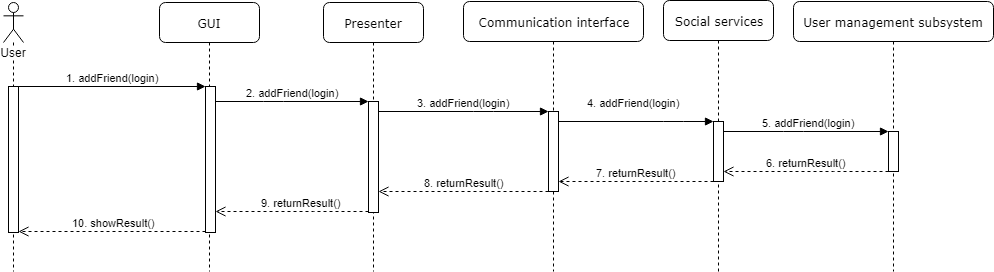
\includegraphics[width=\linewidth]{addFriend}
\caption{Dodanie użytkownika do znajomych.}
\label{fig:addFriend}
\end{figure}

\FloatBarrier
\subsubsection{Zapraszanie użytkownika do aplikacji}

\noindent Warunki początkowe:
\begin{enumerate}
  \item Użytkownik jest zalogowany.
  \item Aplikacja ma dostęp do internetu.
  \item Użytkownik wybrał z menu opcję "Znajomi".
\end{enumerate}
\par
\noindent\newline
Warunki końcowe:
\begin{enumerate}
  \item Wiadomość e-mail została wysłana lub napotkano błąd.
  \item Użytkownik otrzymał informację o pomyślnym wysłaniu zaproszenia lub błędzie.
\end{enumerate}

\noindent\newline
\begin{figure}[h]
\centering
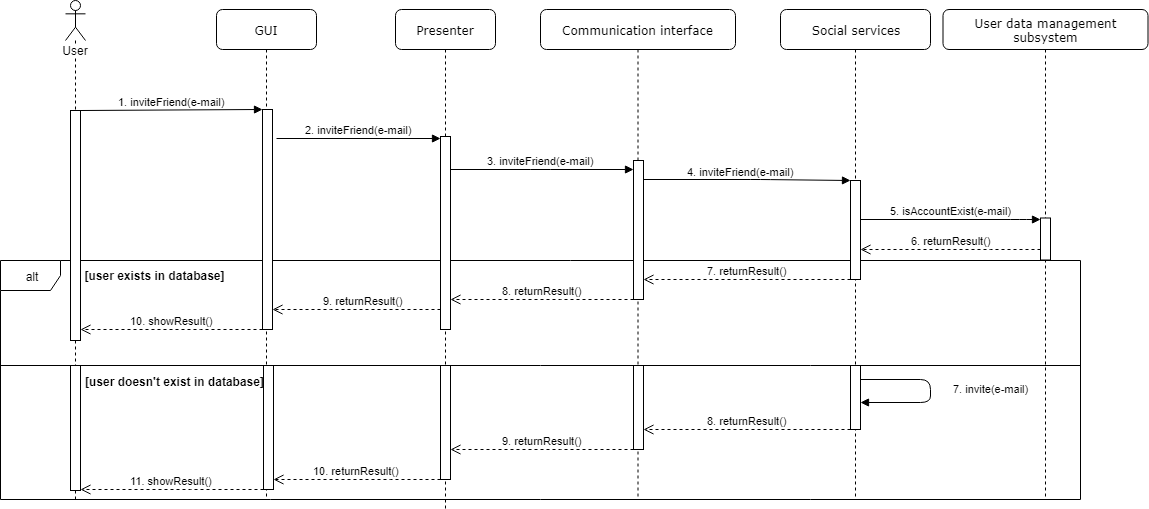
\includegraphics[width=\linewidth]{inviteFriend}
\caption{Zapraszanie użytkownika do skorzystania z aplikacji.}
\label{fig:inviteFriend}
\end{figure}

\FloatBarrier
\subsubsection{Udostępnienie podróży}

\noindent Warunki początkowe:
\begin{enumerate}
  \item Użytkownik jest zalogowany.
  \item Aplikacja ma dostęp do internetu.
  \item Użytkownik wybrał podróż do udostępnienia.
  \item Użytkownik docelowy jest znajomym użytkownika udostępniającego.
\end{enumerate}
\par
\noindent\newline
Warunki końcowe:
\begin{enumerate}
  \item Użytkownik otrzymał informację o rezultacie.
  \item Drugi użytkownik otrzymał informację o udostępnionej podróży.
\end{enumerate}

\noindent\newline
\begin{figure}[h]
\centering
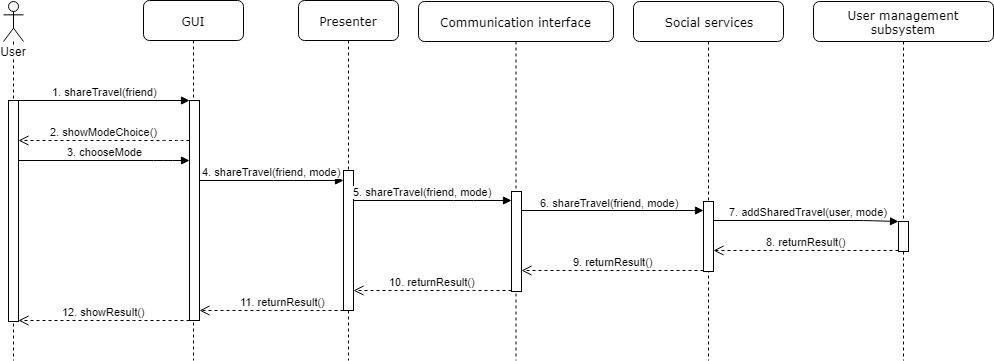
\includegraphics[width=\linewidth]{shareTravel}
\caption{Udostępnienie podróży.}
\label{fig:shareTravel}
\end{figure}


\FloatBarrier
\subsection{Interakcje serwera z aplikacją w czasie trwania podróży (Dorota Tomczak)}
\par Martyna wraz z koleżanką odbywają zaplanowaną poprzez aplikację podróż. W drodze do jednej z atrakcji aplikacja powiadamia Martynę o interesującym obiekcie znajdującym się niedaleko miejsca, w którym przebywają. Dziewczyny ruszają do wskazanej lokalizacji. Tracą poczucie czasu, więc aplikacja informuje je, że jeśli się nie pośpieszą, nie zdążą dojść do następnego punktu planu dnia przed jego zamknięciem (rys.~\ref{fig:whileTravelling}).

\noindent\newline
\begin{figure}[h]
\centering
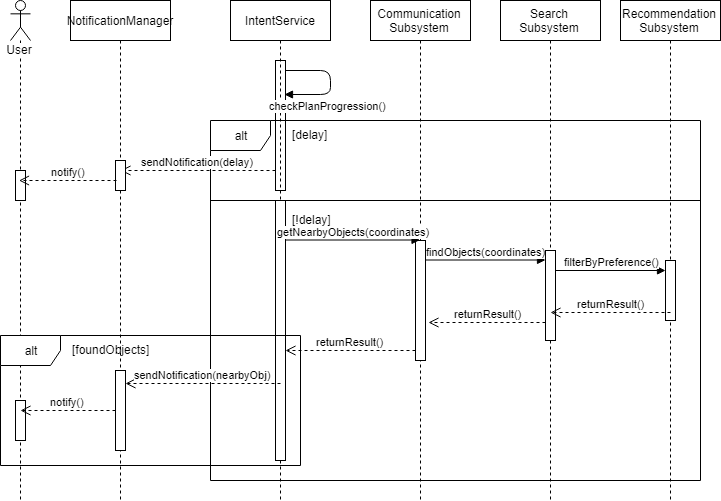
\includegraphics[width=0.9\textwidth]{whileTravelling}
\caption{Otrzymywanie powiadomień podczas trwania podróży.}
\label{fig:whileTravelling}
\end{figure}
\\\\
\noindent\newline Warunki początkowe:
\begin{enumerate}
  \item Użytkownik jest zalogowany.
  \item Aplikacja ma dostęp do internetu.
  \item Aplikacja ma dostęp do lokalizacji użytkownika.
  \item Użytkownik nie zablokował powiadomień od aplikacji.
  \item Użytkownik utworzył plan podróży i jest w określonym miejscu i czasie.
\end{enumerate}

\par
\noindent\newline
Warunki końcowe:
\begin{enumerate}
  \item Użytkownik otrzymał odpowiednie powiadomienie.\\
\end{enumerate}

\FloatBarrier
\subsection{Stworzenie planu podróży (Karolina Makuch)}
\par Martyna pragnie zaplanować podróż za pomocą aplikacji poprzez aplikację podróż.  (rys.~\ref{fig:addTravel}).

\noindent\newline Warunki początkowe:
\begin{enumerate}
  \item Użytkownik jest zalogowany.
  \item Aplikacja ma dostęp do internetu.
  \item Użytkownik wybrał opcję stwórz plan podróży.
\end{enumerate}
\par
\noindent\newline
Warunki końcowe:
\begin{enumerate}
  \item Użytkownik stworzył plan podróży.
\end{enumerate}

\noindent
\begin{figure}[h]
\centering
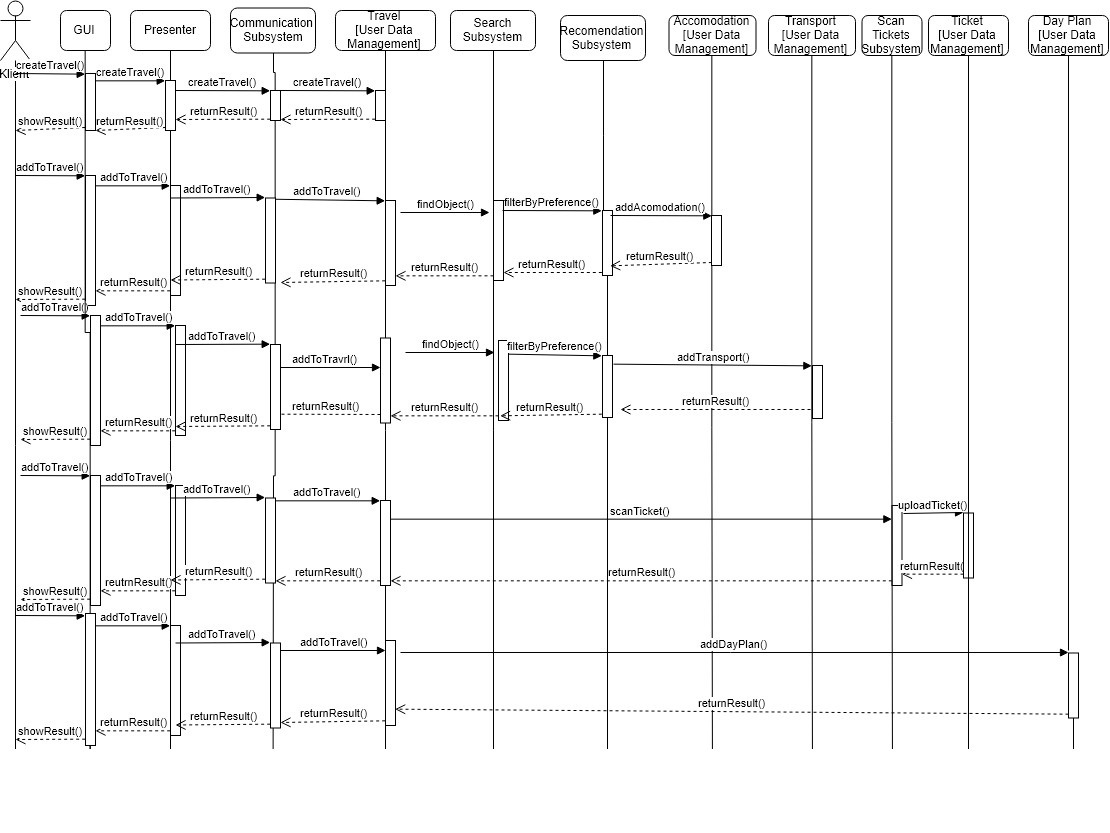
\includegraphics[width=\linewidth]{addTravel}
\caption{Tworzenie planu podróży.}
\label{fig:addTravel}
\end{figure}

\FloatBarrier